\documentclass[twoside,11pt]{article}

% DMLR style (https://github.com/JmlrOrg/dmlr-style-file). Under review the
% preprint option is used, which drops the journal header and editor line.
\usepackage[preprint]{dmlr2e}
\usepackage{booktabs}
\usepackage{amsmath}
\usepackage{url}
\usepackage{multirow}
\usepackage{lastpage}

\newcommand{\gd}[1]{\textbf{#1}}

% Heading arguments: {volume}{year}{pages}{submitted}{published}{paper id}{authors}.
% Filled in by the editors on acceptance.
\dmlrheading{}{2026}{1-\pageref{LastPage}}{}{}{}{Vamsi Vunnam}
\def\openreview{\textit{under review}}
\ShortHeadings{Provenance Confounding in a Phishing E-mail Benchmark}{Vunnam}
\firstpageno{1}

\begin{document}

\title{A Phishing Detector That Never Saw Phishing:\\
Provenance Confounding in a Public Phishing E-mail Benchmark}

\author{\name Vamsi Vunnam \email vunnamvamsi540@gmail.com \\
       \addr University of Arkansas at Little Rock\\
       Little Rock, AR 72204, USA}

\editor{}

\maketitle

\begin{abstract}
Phishing e-mail detectors routinely report accuracy or $F_1$ of 97\% or more
on public benchmarks in which phishing and legitimate mail come from different
collections. We show that on a widely used benchmark of this kind --- Nazario
phishing paired with SpamAssassin ham --- the score can be reproduced from
provenance alone, without any phishing detection. A classifier trained only to
tell two \emph{legitimate} corpora apart, which never sees a phishing label,
scores $F_1$ 98.42\% on the benchmark (97.83\% when its training pool shares
no message with the benchmark; label-shuffled null: 57.34\%); a
pretrained transformer (DeBERTa-v3-small) trained the same way scores
97.84\%. A parameter-free rule, ``phishing if the Date year is 2003 or
later'', scores 99.95\%. A source-exposure sweep shows what the score
measures: a model pooled from three other corpora scores 73.48\%, and adding
50 benchmark e-mails per class raises it to 93.37\%. Decomposing that gain,
false alarms fall mainly when benchmark ham is added and missed phishing falls
mainly when benchmark phishing is added, while fraud e-mails from another
collection barely help. On the six-corpus compilation that is the most
common dataset in our literature audit (82,486 e-mails), provenance does not explain the overall score, but
it governs the phishing slice: a model that never saw the Nazario collection
flags only about 60\% of it, and a year threshold separates Nazario from all
dated legitimate mail with one error in 22,967. We release a tool that runs
these diagnostics on any labelled e-mail collection, and propose that a
source-exposure sweep and a provenance-transfer bound be reported beside
headline scores.
\end{abstract}

\begin{keywords}
  dataset audit, benchmark validity, shortcut learning, provenance
  confounding, phishing e-mail detection
\end{keywords}

\section{Introduction}

Machine learning for security has a long record of evaluations that flatter
their subjects. \citet{sommer2010} argued that intrusion
detection results seldom survive deployment. \citet{arp2022}
catalogued ten recurring pitfalls, including sampling bias and spurious
correlation, and found them widespread. \citet{pendlebury2019} showed that ignoring time inflates malware
classification substantially.

Phishing e-mail detection now exhibits precisely the symptom those works
anticipate. We checked recent detection papers against their publishers'
pages and found at least 20, published 2023--2026, that train and test on
data whose phishing and legitimate classes come from different source
collections and that report a headline accuracy or $F_1$ of 97\% or more
(Appendix~\ref{app:prevalence}). Only two of the twenty clearly report a test on
a different collection. Several authors have noted that performance falls
across datasets~\citep{indepth2025,meajor2025,pajola2025ephishgen,champa2025illusion}.
What has not been done is to measure how much of the reported score the
construction of the benchmark explains.

\paragraph{An observation that started this.}
While building supervised baselines for an unrelated system, a TF--IDF
bag-of-words model fitted on 930 messages in 0.4\,s of single-core CPU time
reached $F_1$ 99.82\% on the widely used Nazario/SpamAssassin pairing. Linear
models over word counts do not solve hard problems that quickly.

\paragraph{The mechanism.}
Public phishing corpora and public ham corpora are separate artefacts,
gathered by different people, at different times, through different
infrastructure. A benchmark that pairs them makes \emph{every} phishing
message come from one collection and \emph{every} legitimate message from
another. Class label and corpus identity become perfectly correlated, so a
model that learns only ``which collection is this?'' scores as well as one
that learns phishing.

\paragraph{This hazard is old, and was previously solved.}
We want to be explicit, because it bears on what we claim. The spam filtering
community identified this problem two decades ago. \citet{cormack2005,cormack2007} built the TREC spam track around a
\emph{chronological single stream} of messages delivered to one server over
one period, with an adjudicated gold standard, specifically so that filters
could not learn the source instead of the property. The discipline they
established is exactly what the corpus pairings now common in phishing
e-mail research abandon.

Our contribution is therefore not the discovery of a hazard but the
demonstration that a specific, heavily used modern benchmark has re-acquired
it, together with the machinery to measure how badly.

\paragraph{Relation to concurrent work.}
While this work was in preparation, Fragility of Phishing Detection
Models~\citep{fragility2026} appeared, reporting on the same six public corpora
that dataset-identification accuracy reaches 0.9722--0.9806 and that top
features include corpus markers, date tokens and header fields. That paper
independently establishes the phenomenon we describe, and we do not claim
priority for it. Our contribution is complementary and narrower: where \citet{fragility2026} shows corpus identity is \emph{learnable}, we measure how
much of a benchmark score it \emph{accounts for}, by transferring a
provenance-only detector onto the phishing task (\S\ref{sec:transfer}),
measuring how the score responds to exposure to the benchmark's own sources
(\S\ref{sec:pooling}), and exhibiting a parameter-free rule that saturates the
benchmark (\S\ref{sec:modelfree}). Readers should treat the two papers as
converging evidence rather than as competing claims.

\paragraph{Contributions.}
\begin{enumerate}\itemsep2pt
\item \textbf{The provenance-transfer test} (\S\ref{sec:transfer}). A
detector trained on two \emph{legitimate} corpora, never exposed to a
phishing label, scores $F_1$ 98.42\%$\pm$0.25 on the phishing benchmark under
a label-free decision rule; a label-shuffled null scores 57.34\%$\pm$7.53.
The result holds when the detector's training pool is made disjoint from the
benchmark, including near-duplicates (97.78\%$\pm$0.37), when the phishing
source is swapped (93.79\% with Nigerian fraud in place of Nazario), and for a
pretrained transformer (97.84\%$\pm$0.51 with DeBERTa-v3-small,
\S\ref{sec:transformer}).

\item \textbf{A source-exposure sweep and decomposition}
(\S\ref{sec:pooling}). A model pooled from three other corpora scores 73.48\%
on the benchmark; 50 benchmark e-mails per class (2.6\% of its training data)
raise it to 93.37\%. Each type of error is removed mainly by examples from that
class's own source collection, and fraud e-mails from a different collection
barely help.

\item \textbf{A label-invariant separability control} (\S\ref{sec:identity}):
corpus identity is recoverable from body text at 95.19\%$\pm$0.64 with the
class label held fixed, against 50.44\%$\pm$1.13 within one corpus.

\item \textbf{A channel ablation and a model-free demonstration}
(\S\ref{sec:probe}, \S\ref{sec:modelfree}): the \emph{Date} header alone
reaches $F_1$ 99.91\% on the pairing versus 63.43\% on a single-source corpus,
and a hand-written threshold on the Date year attains 99.95\% with no fitted
parameters.

\item \textbf{An audit of the six-corpus compilation}, the most common
dataset in our literature audit (\S\ref{sec:compilation}). Provenance does
not explain its overall score, because four of its six sources contain both
classes; it does govern the single-class phishing source inside it.

\item \textbf{Robustness checks} (\S\ref{sec:repair},
\S\ref{sec:independence}): sanitisation costs 0.42 $F_1$ points,
benchmark-trained models fall to 31.15\% on an unseen corpus whose positive
class is spam, and every role
played by CEAS 2008 is repeated with two unrelated corpora.

\item \textbf{A reporting protocol and a released tool}
(\S\ref{sec:protocol}) that runs the diagnostics on any labelled e-mail
collection.
\end{enumerate}

\paragraph{Scope.}
We claim that this benchmark cannot distinguish a detector that has learned
phishing from one that has learned provenance, and that its score tracks
exposure to its two source collections. We do \emph{not} claim that published
detectors encode no phishing-relevant information, and nothing here says that
pooled or multi-source training is harmful in deployment; it says only that
this benchmark cannot see the difference.

\section{Related Work}

\paragraph{Spam filter evaluation: the discipline that was lost.}
\citet{cormack2005} set out corpus-construction requirements
for the TREC spam track: messages must form a chronological sequence from a
single mail stream, and every message must carry an adjudicated judgement
rather than an inherited source label. The TREC 2005 track went further and
rewrote the headers of its spam so that it appeared to be delivered to the
Enron server during the same period as the ham~\citep{cormack2005trec} --- an
explicit repair of the date channel we measure in \S\ref{sec:modelfree}. TREC
2007~\citep{cormack2007} used ham and spam delivered to the same server in the
same period. The design rationale is the one this paper re-derives
empirically. The pairing we audit goes back at least to \citet{fette2007learning}, who evaluated on about 860 messages of the
public phishing corpus against SpamAssassin ham. The TREC literature is
largely uncited in recent phishing e-mail work, which may be how the error
returned.

\paragraph{Dataset bias, shortcuts and benchmark reliability.}
That datasets carry recognisable signatures is an old observation in
vision~\citep{torralba2011}, and it persists for modern networks on large,
supposedly unbiased collections~\citep{liu2025decade}. \citet{geirhos2020} give the general account of shortcut learning; in text
classification, style and occurrence shortcuts have been catalogued
systematically~\citep{zhou2024shortcut}. Benchmark scores also depend on the
specific collection: re-collecting a test set with the same protocol lowers
accuracy~\citep{recht2019imagenet}, label errors in test sets can reorder
models~\citep{northcutt2021pervasive}, and leakage between training and
evaluation data has caused reproducibility failures across
fields~\citep{kapoor2023leakage}. \citet{paullada2021data}
survey these problems in dataset development and use, and WILDS~\citep{koh2021wilds}
shows that shifts across sources and time degrade models that look strong
in-distribution. Our instruments are dataset audits in this tradition: the
label-invariant control adapts Torralba and Efros by holding the label fixed,
and the source-exposure sweep measures how much of a score is bought by
familiarity with the evaluation collections.

\paragraph{Dataset documentation and provenance.}
Datasheets~\citep{gebru2021datasheets} and data cards~\citep{pushkarna2022datacards}
ask dataset creators to record collection process and composition --- exactly
the information that would have exposed this confound. A large audit of
dataset licensing found that licences on hosting sites are frequently missing
or miscategorised~\citep{longpre2024audit}; we find the same in the lineage of
the phishing compilation (see the Data Availability section).

\paragraph{Pitfalls in security ML.}
\citet{arp2022} name sampling bias and spurious correlation among
ten pitfalls and document their prevalence. \citet{pendlebury2019} formalise temporal bias for malware and give
constraints that remove it. Our work instantiates both for a named benchmark
and adds a test that attributes a specific quantity of measured performance to
the confound rather than merely flagging its possibility.

\paragraph{Partial-input baselines and site confounding.}
NLI benchmarks proved substantially solvable from the hypothesis
alone~\citep{gururangan2018,poliak2018}, and chest-radiograph models learned to
identify the hospital, whose disease prevalence confounded the
label~\citep{zech2018}. The provenance-transfer test is a partial-input
baseline of this kind taken to its limit: it extends ``the dataset is
identifiable'' to ``identifying the dataset solves the task'' by training on
no example of the positive class at all.

\paragraph{Phishing e-mail evaluation.}
The closest prior work is Fragility of Phishing Detection
Models~\citep{fragility2026}, published shortly before this study was completed.
Using the same six public corpora, it reports dataset-identification accuracy
of 0.9722 (logistic regression) and 0.9806 (linear SVC), identifies corpus
markers, date tokens and header fields among top features, and evaluates
artefact-removal ablation and cross-corpus transfer. It further examines
prevalence shift and evasion, which we do not. We regard our work as
complementary: it shares the diagnosis and differs in instrument. The
provenance-transfer test, the source-exposure sweep and its decomposition, and
the parameter-free demonstration are, to our knowledge, not present in that
work, and they answer a different question --- not whether
corpus identity is learnable, but how much of a reported score it explains.
\citet{champa2025illusion}, who curated the collection from
which the six-corpus compilation appears to derive, reassess machine-learning
phishing detectors and find that performance varies substantially on unseen
or recent e-mails; they attribute the drop mainly to the age of the training
data. Our account differs in emphasis and in instrument. In these corpora
collection and era are confounded, so the two explanations overlap; we hold
the class fixed and show that the collections themselves are separable
(\S\ref{sec:identity}), estimate the contribution of drift within a single
collection and find it smaller than the cross-collection effect
(Table~\ref{tab:drift}), and show that a detector with no phishing labels
reproduces the benchmark score (\S\ref{sec:transfer}).
E-PhishGen~\citep{pajola2025ephishgen} reports near-perfect
within-dataset scores that collapse across datasets and responds by generating
new data with language models; we audit the existing data instead.
Surveys report cross-dataset degradation and inconsistent
benchmarks~\citep{indepth2025,meajor2025}; website-phishing work has questioned
benchmark construction~\citep{website2020}. Closest in time to our work,
PhishFuzzer~\citep{phishfuzzer2026} constructs a new synthetic benchmark with
explicit provenance tracking and observes that LLM detector performance is
sensitive to metadata inclusion and to whether seeds are drawn from private or
public corpora --- observations consistent with our findings, approached from
the construction side rather than the audit side. We are not aware of prior
work that applies a provenance-transfer or label-invariant control to existing
phishing e-mail corpora, or that attributes their reported accuracies to
corpus composition.

\section{Framework and Methodology}
\label{sec:method}

\subsection{Definitions}

Let a corpus $C$ be a set of messages with a provenance tag $s(x)=C$ and a
class label $y(x)\in\{\textsc{benign},\textsc{phish}\}$. A benchmark
$B=C_1\cup C_2$ is \emph{provenance-confounded} when $s$ determines $y$:
every message from $C_1$ is phishing and every message from $C_2$ is benign.
Under that condition any classifier of $s$ is also a classifier of $y$ with
identical error, so no evaluation on $B$ can separate a model that has learned
$y$ from one that has learned $s$.

We quantify the confound with three instruments of increasing strength.

\paragraph{(I1) Channel ablation.}
Fit a classifier on a \emph{view} $v(x)$ --- a projection of the message onto
a subset of its content --- and record test performance. Views that retain no
persuasive content but still separate the classes indicate a leaking channel.
Ablation alone is suggestive, not conclusive: a view may carry genuine signal.
Every ablation result is therefore reported beside a single-source control
corpus, in which $s$ does not determine $y$.

\paragraph{(I2) Label-invariant separability.}
Fix $y$ and predict $s$. Formally, sample $A\subset C_1$ and $B\subset C_2$
with $y(x)=c$ for all $x\in A\cup B$, and measure how well $s$ is recoverable.
Because $y$ is constant, accuracy above chance cannot arise from class signal.
The pair must be chosen so that no \emph{sub-class} difference substitutes for
it; we return to this in \S\ref{sec:identity}. A within-corpus null (split one
corpus at random, predict which half) establishes that the procedure creates
no separability of its own.

\paragraph{(I3) Provenance transfer.}
The strongest instrument, and the one we contribute. Train a provenance
detector $P$ on a pair of corpora that share a class label, so $P$ observes no
class supervision. Apply $P$ unchanged to the benchmark, and convert its
provenance prediction into a class prediction with a fixed rule derived only
from how the benchmark was assembled:
\[
\hat{y}(x)=
\begin{cases}
\textsc{benign} & \text{if } \hat{s}(x)=C_{\text{ham source}}\\
\textsc{phish}  & \text{otherwise.}
\end{cases}
\]
Score $\hat{y}$ against the benchmark's own ground truth. One side of the pair
is the benchmark's own ham source; the other is a stand-in for ``not that
source'', drawn from a corpus that appears nowhere in the benchmark. $P$ never
sees the benchmark's phishing source, so on that side the resulting $F_1$ is a
\emph{lower bound} on how much of a reported score corpus construction can
account for. Because the ham-side pool comes from the same corpus as the
benchmark's ham, it can contain benchmark test messages; we therefore report
every transfer figure both as constructed and with the training pool made
disjoint from the evaluation set (\S\ref{sec:overlap}). A label-shuffled null
verifies that any performance comes from the learned provenance signal rather
than from the mapping.

\subsection{Experimental Setup}

\paragraph{Corpora.} Nazario phishing~\citep{nazario_corpus} (2015--2022 by
Date header), the SpamAssassin public corpus~\citep{spamassassin_corpus}
(2000--2002, ham and spam), the CLAIR Nigerian fraud
collection~\citep{radev2008clair} (mostly 2005--2007), and the CEAS 2008
challenge corpus~\citep{ceas2008_corpus}; the pooled experiments and the
compilation audit add Ling-Spam~\citep{androutsopoulos2000lingspam} and
Enron~\citep{klimt2004}. CEAS matters because it carries both classes from one
collection, giving a corpus in which $s$ does not determine $y$.

\paragraph{Benchmark.} Following common practice we pair Nazario phishing with
SpamAssassin ham, deduplicate on a hash of sender, subject and body prefix,
drop messages under 30 body characters or lacking a sender, and balance the
classes: 3{,}100 messages. A stratified 30/70 split is drawn with a fixed seed. The
smaller partition serves as the \emph{training} set for every fitted model and
for any hyper-parameter choice; the larger is held out and scored once. We
chose the unusual direction deliberately, to obtain a precise held-out
estimate. It gives the supervised reference less training data than usual;
the provenance detector does not use this partition at all.

\paragraph{Classifier.} TF--IDF over word unigrams and bigrams
($\min\text{df}=2$, sublinear term frequency, $\leq 2\times10^5$ features)
with $\ell_2$-regularised logistic regression ($C=4$, balanced class weights).
The model is deliberately weak: a simple model saturating a benchmark is
stronger evidence of a shortcut than a large one doing so. We repeat the key
experiments with a pretrained transformer (\S\ref{sec:transformer}).

\paragraph{Statistics.} Every figure reported with $\pm$ is a mean over
five random seeds with the half-width of a 95\% Student-$t$ interval
($t_{0.975,4}=2.776$); cross-validated figures use 5 folds. Figures without
$\pm$ --- the supervised reference, the channel ablation and model-family
tables, sanitisation and cross-corpus rows, and leave-one-source-out results
--- are single runs. We state plainly
what this interval covers: the seeds resample from a \emph{fixed} corpus, so
the interval quantifies sampling variability within these corpora and not
generalisation to corpora we did not observe. The latter is addressed by
\S\ref{sec:generalise} and \S\ref{sec:compilation} rather than by any
interval. Where a condition uses the entire training partition, the seed does
not change the training set and the interval is zero; we mark such cells.
Where we compare conditions the separations are large relative to this
variability --- the provenance detector and its null differ by roughly 41
points with non-overlapping intervals, and 95.19\% versus 50.44\% in
Table~\ref{tab:identity} likewise --- so we report effect sizes rather than
$p$-values, which would be uninformative at these magnitudes. Timings are
single-core on a 2.4\,GHz x86-64 container. The TF--IDF experiments were
reproduced on a second machine (Python 3.9.6, scikit-learn 1.6.1,
NumPy 2.0.2).

\section{Provenance Transfer}
\label{sec:transfer}

\paragraph{Construction.}
We train $P$ to distinguish SpamAssassin ham from CEAS ham. Both sides are
legitimate mail, so $P$ receives no phishing supervision of any kind and
cannot represent phishing except by accident. We then apply $P$ to the
benchmark \emph{test} split and map its output through the fixed rule of
\S\ref{sec:method}: messages judged to resemble SpamAssassin are predicted
benign, all others phishing. The mapping encodes no property of phishing; it
encodes only the fact that the benchmark drew its ham from SpamAssassin.

\begin{table}[t]
\centering\small
\caption{Provenance transfer. A detector trained only on two \emph{legitimate}
corpora, evaluated as a phishing detector on the benchmark test split
($n=2{,}170$). Mean over five seeds, $\pm$ 95\% Student-$t$ half-width. MCC and
balanced accuracy are reported because $F_1$ on a balanced set rewards a
classifier that simply favours the positive class.}
\label{tab:transfer}
\begin{tabular}{lrrrr}
\toprule
Condition & $F_1$ & Bal.\ acc. & MCC & \% called phish \\
\midrule
\emph{Trivial: always phishing} & 66.67 & 50.00 & 0.000 & 100.0 \\
Null (provenance labels shuffled) & 57.34\,$\pm$7.53 & 55.21\,$\pm$5.93 & 0.106 & 55.4 \\
\gd{Provenance detector} & \gd{98.42}\,$\pm$0.25 & \gd{98.40}\,$\pm$0.26 & \gd{0.968} & 51.4 \\
\midrule
\emph{Reference:} supervised TF--IDF & 99.82 & 99.82 & 0.996 & 49.9 \\
\bottomrule
\end{tabular}
\end{table}

\paragraph{Result.}
Table~\ref{tab:transfer}. The provenance detector reaches $F_1$
98.42\%$\pm$0.25, within 1.4 points of a fully supervised classifier trained
with phishing labels on the benchmark itself.

Two comparison points matter. First, the correct floor for $F_1$ on a balanced
binary task is not 50\% but 66.67\%, attained by a constant classifier; we
include it because the label-shuffled null (57.34\%) falls \emph{below} it and
would otherwise flatter our result. Second, the provenance detector is not
merely biased toward the positive class: it labels 51.4\% of the test set
phishing against a true rate of 50.0\%, and attains MCC 0.968 and balanced
accuracy 98.40\%, so the figure is not an artefact of class-prior exploitation.

\paragraph{Reading it.}
Knowing only how the benchmark was assembled --- not what phishing is ---
suffices to solve it. On the phishing side this is a lower bound: $P$ never saw
Nazario, and CEAS ham merely stands in for ``not SpamAssassin''; a detector
trained on the benchmark's own phishing source would do at least as well.
Reported scores on this benchmark therefore cannot be read as evidence of
detection ability, because a system with no such ability attains them.

\paragraph{Overlap with the evaluation set.}
\label{sec:overlap}
The ham side of $P$'s training pool is drawn from the SpamAssassin corpus,
which also supplies the benchmark's ham. Of the 1{,}085 ham messages in the
test split, 1{,}037 (95.6\%) are in that pool, and with 1{,}500 drawn per seed
from 4{,}091 roughly a third of them are seen in training. The overlap is
intrinsic to the construction --- recognising SpamAssassin is what $P$ is for
--- but it must not be the mechanism. Table~\ref{tab:overlap} repeats the test
with every benchmark message (development and test) removed from the pool,
and again after also removing pool messages whose word 5-shingle Jaccard
similarity to any benchmark message is at least 0.8. The pool shrinks from
4{,}091 to 2{,}605 and then 2{,}543 messages; $F_1$ moves from 98.42\% to
97.83\% and 97.78\%, and the share of messages called phishing stays at
51--52\%. Memorised messages contribute well under a point. The same holds for
the composed benchmarks of \S\ref{sec:generalise}, where the ham source is
split into disjoint halves for training and evaluation.

\begin{table}[t]
\centering\small
\caption{Overlap control. Provenance-transfer $F_1$ (\%) as constructed and
with $P$'s training pool made disjoint from the evaluation messages (exact
copies removed; then near-duplicates with 5-shingle Jaccard $\geq 0.8$ also
removed). For the composed benchmarks the ham source is split in two with an
independent random seed. Mean $\pm$ 95\% Student-$t$ half-width over five
seeds.}
\label{tab:overlap}
\begin{tabular}{lrrr}
\toprule
Benchmark & As constructed & Exact-disjoint & Near-disjoint \\
\midrule
Benchmark test split & 98.42\,$\pm$0.25 & 97.83\,$\pm$0.32 & 97.78\,$\pm$0.37 \\
\quad balanced accuracy & 98.40 & 97.79 & 97.73 \\
\quad MCC & 0.968 & 0.956 & 0.955 \\
\quad label-shuffled null $F_1$ & 57.34\,$\pm$7.53 & 51.86\,$\pm$20.28 & 48.15\,$\pm$19.78 \\
\midrule
Composed: Nazario / SpamAssassin ham & 98.29\,$\pm$0.58 & 97.51\,$\pm$0.49 & 97.36\,$\pm$0.49 \\
Composed: Nigerian / SpamAssassin ham & 93.79\,$\pm$2.70 & 92.41\,$\pm$3.85 & 93.35\,$\pm$1.25 \\
\bottomrule
\end{tabular}
\end{table}

\begin{figure*}[t]
\centering
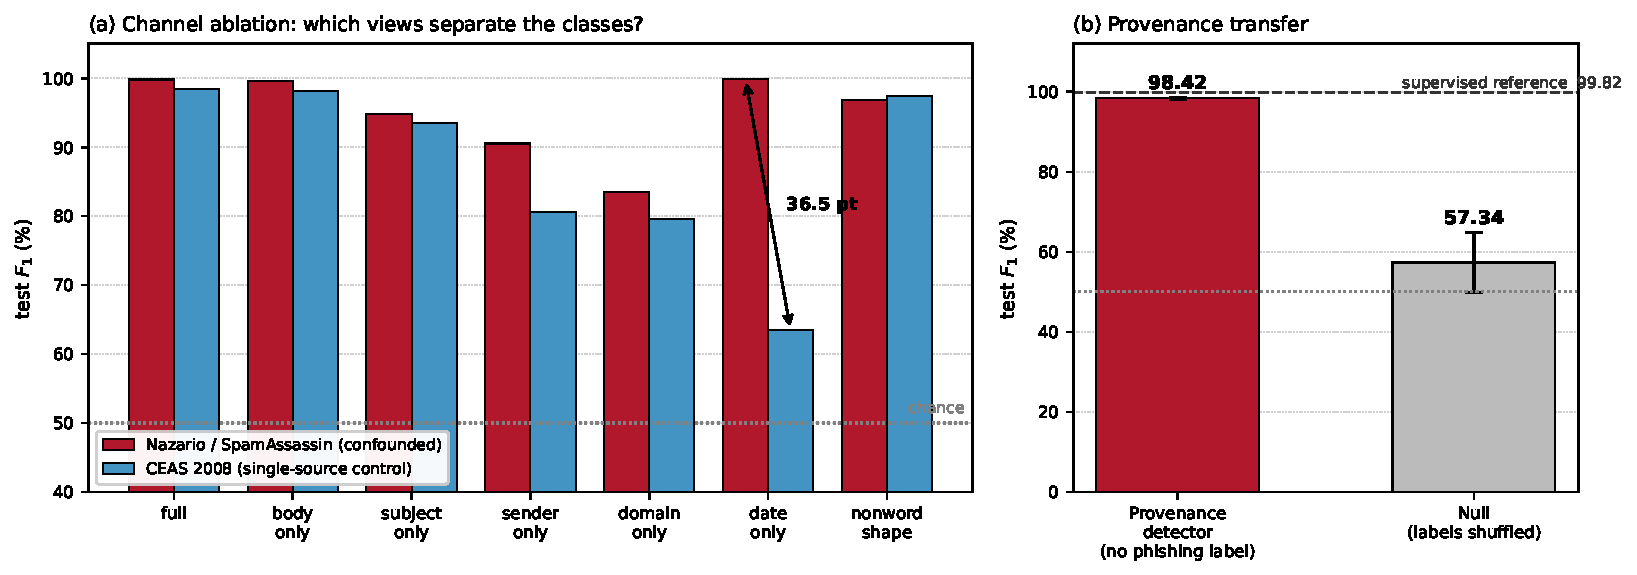
\includegraphics[width=\textwidth]{fig1.pdf}
\caption{(a) Channel ablation. Views retaining no persuasive content still
separate the confounded pairing; the 36.5-point gap on \texttt{date\_only}
against the single-source control is the confound made visible. (b) A detector
trained only on two \emph{legitimate} corpora, never exposed to a phishing
label, reaches within 1.4 points of a supervised classifier on the phishing
benchmark. Error bars in (b) are 95\% Student-$t$ half-widths over five
seeds; panel (a) shows single runs.}
\label{fig:main}
\end{figure*}

\subsection{Does It Generalise Beyond One Benchmark?}
\label{sec:generalise}

We repeat the test on five benchmarks composed from different source
combinations (Table~\ref{tab:generalise}). The result is instructive precisely
because it is not uniform.

\begin{table}[t]
\centering\small
\caption{Provenance transfer across composed benchmarks. Mean $\pm$ 95\%
Student-$t$ half-width over five seeds.
The provenance detector is always trained on the benchmark's own ham source
versus a stand-in corpus, and never sees a phishing label. In this table the
training pool and the benchmark's ham are sampled from the same list;
Table~\ref{tab:overlap} repeats the two SpamAssassin-ham rows with disjoint
halves.}
\label{tab:generalise}
\begin{tabular}{lrr}
\toprule
Benchmark (phishing / ham) & Transfer $F_1$ & Null $F_1$ \\
\midrule
\gd{Nazario / SpamAssassin ham}  & \gd{98.29}\,$\pm$0.58 & 51.66\,$\pm$13.78 \\
\gd{Nigerian / SpamAssassin ham} & \gd{93.79}\,$\pm$2.70 & 48.23\,$\pm$18.24 \\
\midrule
Nazario / CEAS ham               & 0.22\,$\pm$0.19  & 53.83\,$\pm$18.22 \\
Nigerian / CEAS ham              & 15.48\,$\pm$9.78 & 57.17\,$\pm$20.05 \\
SpamAssassin spam / CEAS ham     & 58.41\,$\pm$6.71 & 54.13\,$\pm$11.46 \\
\bottomrule
\end{tabular}
\end{table}

Transfer succeeds on both benchmarks whose ham side is SpamAssassin --- the
construction used by the benchmark we study --- reaching
98.29\% and 93.79\% with two \emph{different} phishing sources. That the
phishing side can be swapped with the result largely intact (98.29\% to
93.79\%) indicates that the benchmark's difficulty resides mainly in the ham
side's provenance.

It fails when the ham side is CEAS, and we can show why rather than assert
it. A detector trained to separate CEAS ham from SpamAssassin assigns
99.9\%$\pm$0.1 of Nazario messages to the CEAS class, and therefore calls them
benign. (In the SpamAssassin-spam row the transfer and null intervals overlap,
so that row is indistinguishable from chance.) The Nazario/SpamAssassin row
is a separate run with its own sampling, so it differs slightly from
Table~\ref{tab:transfer} (98.29\% versus 98.42\%). Nazario resembles neither training corpus; it is out of distribution,
and the decision boundary places it almost entirely on one side. The failure
is a property of the proxy, not evidence against the confound. We report it
because the directionality is itself informative --- had transfer succeeded
everywhere, that would point to an artefact of our method rather than to a
property of these corpora.

\subsection{Robustness to Model Family}
\label{sec:families}

All other results use logistic regression. Table~\ref{tab:families} repeats
the channel ablation across six estimator families spanning margin,
probabilistic, ensemble and neural approaches.

\begin{table}[t]
\centering\small
\caption{Channel ablation across model families. Test $F_1$ (\%). The profile
is a property of the data, not of the estimator.}
\label{tab:families}
\begin{tabular}{lrrrr}
\toprule
Model & \texttt{full} & \texttt{body} & \gd{\texttt{date}} & \texttt{domain} \\
\midrule
Logistic regression        & 99.82 & 99.63 & \gd{99.91}  & 83.54 \\
LinearSVC (margin)         & 99.86 & 99.77 & \gd{100.00} & 83.49 \\
ComplementNB (probabilistic)& 99.72 & 99.40 & \gd{99.40}  & 75.95 \\
SGD, hinge loss            & 99.91 & 99.72 & \gd{100.00} & 84.65 \\
HistGradientBoosting       & 99.68 & 99.72 & \gd{98.52}  & 85.02 \\
MLP $1\times256$ (from scratch) & 99.72 & 99.63 & \gd{99.95} & 84.58 \\
\bottomrule
\end{tabular}
\end{table}

Every family reproduces the profile, and two reach $F_1$ 100.00\% from the
Date header alone. None of these is pretrained; we turn to that next.

\subsection{A Pretrained Transformer}
\label{sec:transformer}

Pretrained transformers are widely used on these corpora
(Appendix~\ref{app:prevalence}), so we repeat the provenance-transfer test and the cross-corpus check with
DeBERTa-v3-small, fine-tuned for three epochs (learning rate
$2\times10^{-5}$, batch size 16, maximum length 384 tokens) over five seeds,
on exactly the provenance training sets used for the TF--IDF detector (1{,}500
messages per side). Two implementation details are reported for
reproducibility: the checkpoint loaded in half precision, so the model was cast
to single-precision master weights before mixed-precision training; and the
run used eager rather than scripted kernels (\texttt{PYTORCH\_JIT=0}) because
the GPU runtime lacked a library the scripted kernels require. Runs used
transformers 5.17.0 and PyTorch 2.11.0 on an NVIDIA T4.

\begin{table}[t]
\centering\small
\caption{Pretrained transformer (DeBERTa-v3-small) versus the TF--IDF
detector. $F_1$ (\%), mean $\pm$ 95\% Student-$t$ half-width over five
seeds. The cross-corpus column is scored on 4{,}000 CEAS 2008 messages (2{,}000
per class).}
\label{tab:transformer}
\begin{tabular}{lrr}
\toprule
Check & DeBERTa-v3-small & TF--IDF + LR \\
\midrule
Supervised, benchmark test split & 99.43\,$\pm$0.22 & 99.82 \\
Supervised, cross-corpus (CEAS 2008) & 50.90\,$\pm$9.99 & 31.15 \\
\gd{Provenance detector (no phishing labels)} & \gd{97.84}\,$\pm$0.51 & \gd{98.42}\,$\pm$0.25 \\
\quad training pool disjoint from benchmark & 97.40\,$\pm$0.42 & 97.83\,$\pm$0.32 \\
Null (provenance labels shuffled) & 59.58\,$\pm$7.98 & 57.34\,$\pm$7.53 \\
\bottomrule
\end{tabular}
\end{table}

The result carries over (Table~\ref{tab:transformer}). Trained only to tell
SpamAssassin ham from CEAS ham, the transformer scores $F_1$ 97.84\% on the
phishing benchmark, within 1.6 points of the same architecture trained with
phishing labels (99.43\%), while its shuffled-label null falls to 59.58\%. The
upper end of that null's interval (67.56\%) slightly exceeds the 66.67\%
constant-classifier floor, but it lies about 30 points below the provenance
detector. The supervised transformer also loses about half its score on an unseen
corpus (50.90\%, with seeds ranging from 41 to 60), although that corpus's
positive class is spam rather than phishing, so part of this drop is a change
of task. Pretraining therefore does
not remove the confound: a pretrained model given only provenance supervision
still solves the benchmark. The transformer was first trained on the same
provenance pool as the TF--IDF detector, which overlaps the benchmark's ham
(\S\ref{sec:overlap}). With every benchmark message removed from that pool
(4{,}091 to 2{,}605 messages) it scores 97.40\%$\pm$0.42, a fall of 0.4
points, comparable to the 0.6-point fall for TF--IDF; an independent repeat of
the same five seeds gave 97.24\%$\pm$0.65. These reruns used transformers
5.22.0 on the same GPU type; their label-shuffled null was not completed. We ran one small
transformer and did not repeat the source-exposure sweep of
\S\ref{sec:pooling} with it.

\section{What the Benchmark Score Measures: Source Exposure}
\label{sec:pooling}

Concurrent work~\citep{fragility2026} recommends \emph{pooled multi-corpus
training} as a mitigation for artefact learning. We test it on this
benchmark, and use the result to measure directly what the benchmark score
responds to.

\paragraph{Setup.} We build a pool from three corpora that each contribute
\emph{both} classes --- CEAS, Ling-Spam and Enron, 3{,}716 messages in total,
balanced by class --- so that within the pool corpus identity does not
determine the label. The pool's positive class is spam rather than phishing,
because we know of no public collection that supplies both phishing and
legitimate mail from one stream. We then add $k$ messages per class from the benchmark's own
training partition (``dev'', 465 per class) and score every model on the
unchanged benchmark test split (2{,}170 messages), over five seeds. To see
which added messages matter, we also add dev ham only, dev phishing only, or
Nigerian fraud messages from a different collection as positives.

\begin{figure*}[t]
\centering
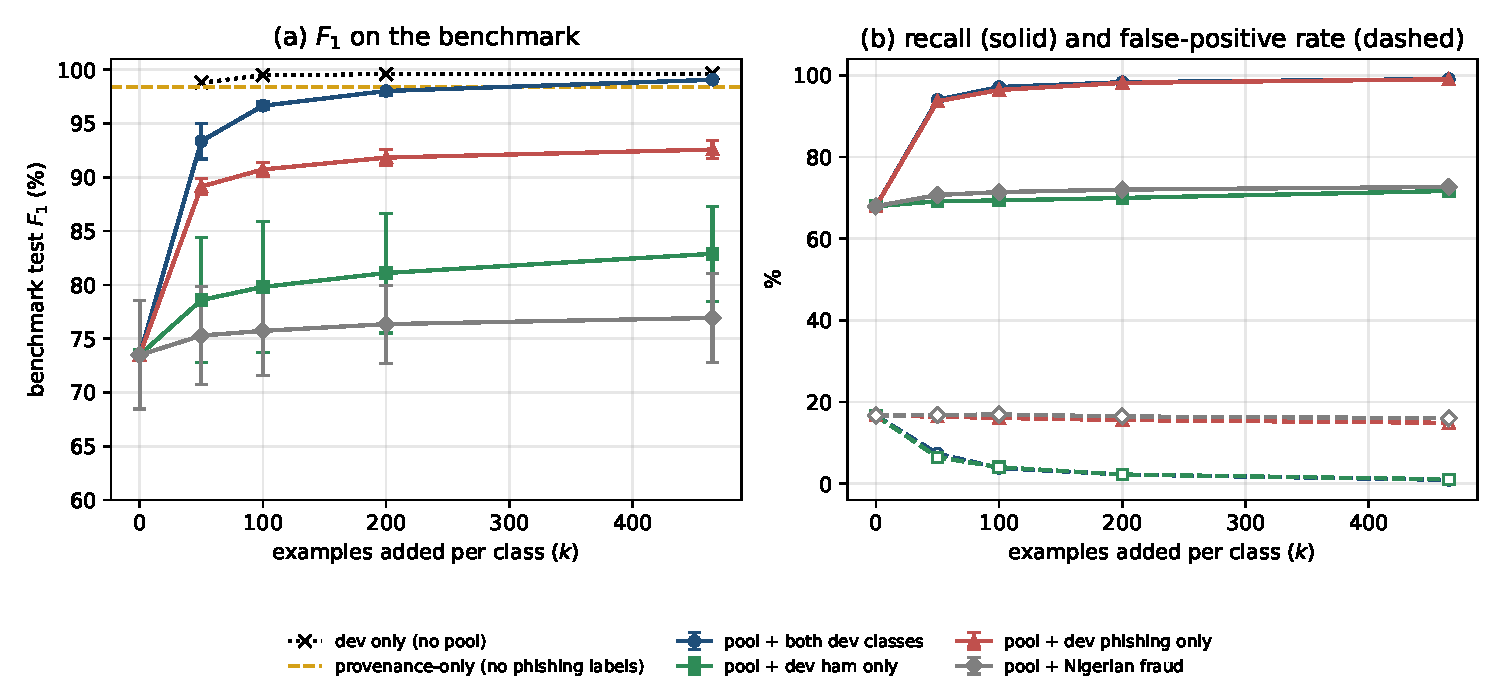
\includegraphics[width=\textwidth]{fig_source_exposure.pdf}
\caption{Source exposure. (a) Benchmark $F_1$ as $k$ messages per class are
added to the pool; the dashed line is the provenance-only detector, which
never sees a phishing label. (b) Recall (solid) and false-positive rate
(dashed) for the same arms. Error bars in (a) are 95\% Student-$t$
half-widths over five seeds.}
\label{fig:exposure}
\end{figure*}

\begin{table}[t]
\centering\small
\caption{Source-exposure sweep and decomposition. A pooled model (CEAS,
Ling-Spam and Enron; 3{,}716 messages whose positive class is spam) is trained
with $k$ additional messages of the kind named in each column: $k$ per
class from the benchmark's own training partition (``dev'', 465 per class),
$k$ dev ham only, $k$ dev phishing only, or $k$ Nigerian fraud messages as
positives. The last column trains on dev messages alone, without the pool.
All models are scored on the unchanged benchmark test split ($n=2{,}170$),
which shares no message body with dev or with the Nigerian sample. Values are
$F_1$ (\%), mean $\pm$ 95\% Student-$t$ half-width over five seeds. The
dev-only cell at $k=465$ has no interval because it uses the whole dev
partition, so the seed does not change the training set.}
\label{tab:source_exposure}
\begin{tabular}{rccccc}
\toprule
 & \multicolumn{4}{c}{Pool (CEAS + Ling + Enron) plus $k$ per class of \ldots} & \\
\cmidrule(lr){2-5}
$k$ & both dev classes & dev ham only & dev phishing only & Nigerian fraud & dev only \\
\midrule
0 & 73.48\,$\pm$5.02 & --- & --- & --- & --- \\
50 & 93.37\,$\pm$1.67 & 78.59\,$\pm$5.85 & 89.15\,$\pm$0.74 & 75.29\,$\pm$4.57 & 98.79\,$\pm$0.40 \\
100 & 96.65\,$\pm$0.35 & 79.81\,$\pm$6.05 & 90.73\,$\pm$0.67 & 75.72\,$\pm$4.15 & 99.49\,$\pm$0.11 \\
200 & 98.02\,$\pm$0.38 & 81.10\,$\pm$5.57 & 91.83\,$\pm$0.73 & 76.35\,$\pm$3.63 & 99.59\,$\pm$0.11 \\
465 & 99.07\,$\pm$0.09 & 82.89\,$\pm$4.43 & 92.58\,$\pm$0.83 & 76.93\,$\pm$4.15 & 99.63\,$\pm$0.00 \\
\midrule
\multicolumn{6}{l}{Provenance-only detector (no phishing labels): 98.42\,$\pm$0.25} \\
\midrule
\multicolumn{6}{l}{\emph{Error split at $k=465$ (recall / false-positive rate, \%):}} \\
\multicolumn{6}{l}{\quad both dev classes: 99.06 / 0.92} \\
\multicolumn{6}{l}{\quad dev ham only: 71.67 / 1.07} \\
\multicolumn{6}{l}{\quad dev phishing only: 99.00 / 14.88} \\
\multicolumn{6}{l}{\quad Nigerian fraud: 72.65 / 16.02} \\
\multicolumn{6}{l}{\quad pool only ($k=0$): 67.93 / 16.66} \\
\bottomrule
\end{tabular}
\end{table}


\paragraph{Result 1: pooling removes the date shortcut but scores 73.48\%.}
A pooled model given only the Date field scores $F_1$ 49.12\%$\pm$4.58, so
pooling across corpora that each supply both classes does remove the date
artefact, as \citet{fragility2026} argue. The same pooled model, given the
full message, scores 73.48\%$\pm$5.02 on the benchmark (recall 67.93\%,
false-positive rate 16.66\%) --- far below the provenance-only detector
(98.42\%).

\paragraph{Result 2: a small amount of source exposure buys most of the
score.} Adding 50 benchmark messages per class --- 100 messages, 2.6\% of the
training data --- raises $F_1$ from 73.48\% to 93.37\%$\pm$1.67
(Table~\ref{tab:source_exposure}, Figure~\ref{fig:exposure}a). At $k=100$ it
reaches 96.65\%, at $k=200$ 98.02\%, and with the whole dev partition 99.07\%.
Training on dev alone, with no pool, gives 98.79\% at $k=50$ and 99.63\% at
$k=465$.

\paragraph{Result 3: each error is removed mainly by its own source.} Is the
pooled model low simply because it never saw phishing? The decomposition
answers this (Table~\ref{tab:source_exposure}, error split, and
Figure~\ref{fig:exposure}b). Because $F_1$ is computed on the phishing class
it weighs missed phishing more heavily than false alarms, so we count errors
on the 1{,}085 messages per class of the test split. The pool alone misses
about 348 phishing messages and raises about 181 false alarms. Adding 465
dev \emph{ham} messages --- which carry no information about phishing at all
--- removes about 169 of the 181 false alarms (false-positive rate 16.66\%
$\to$ 1.07\%) while recall stays near 72\%. Adding 465 dev \emph{phishing}
messages raises recall from 67.93\% to 99.00\% while the false-positive rate
stays near 15\%. Adding 465 Nigerian fraud messages from a different
collection changes almost nothing (recall 72.65\%, false-positive rate
16.02\%). In balanced accuracy the gains over the pool are 9.67 points for
dev ham, 16.43 for dev phishing, 2.68 for Nigerian fraud and 23.44 for both
dev classes together. The phishing side gains more because the pool's largest
error was missed phishing, not because phishing examples are worth more per
message.

\paragraph{Result 4: the gain is not near-copies.} The split was
de-duplicated on a hash of sender, subject and body prefix, and no body occurs
in both partitions, but phishing campaigns reuse templates. Measured by word
5-shingle Jaccard similarity, 71 of the 1{,}085 test phishing messages (6.5\%)
have a development-set neighbour at $\geq 0.8$ and 158 (14.6\%) at
$\geq 0.5$; for ham the counts are 7 and 28. We therefore removed every
development message with a test neighbour at $\geq 0.5$ (117 phishing, 24 ham)
and reran the sweep with the same seeds. The curve is unchanged within its
interval: 93.46\% at $k=50$ (originally 93.37\%), 96.44\% at $k=100$ (96.65\%),
98.15\% at $k=200$ (98.02\%), and 98.84\% with all 348 remaining messages per
class. The steep rise at small $k$ is familiarity with the collections, not
recall of specific messages.

\paragraph{Reading.} Put the two ends of Table~\ref{tab:source_exposure} side
by side. A detector with no phishing labels scores 98.42\%; a detector
trained on all 465 benchmark examples per class scores 99.63\%. Phishing
labels add about 1.2 points; adding the benchmark's own examples to the pool
adds about 26 (73.48\% $\to$ 99.07\%). The ham half of that gain
is clearly source exposure, since the added messages contain no phishing. The
phishing half cannot be split into ``Nazario source'' and ``phishing content'',
because the only phishing we can add is Nazario's; that fraud messages from
another collection barely help argues for source, subject to the caveat that
advance-fee fraud is not credential phishing.

\paragraph{Consequence.} Pooling is a \emph{training-side} intervention;
provenance confounding is an \emph{evaluation-side} property. A researcher
who adopts pooling and then reports on this benchmark will see the model
score lower and may conclude that the intervention failed, when the benchmark
is measuring exposure to its own two collections. Nothing here shows that
pooled training is worse in deployment; it shows that this benchmark cannot
see its benefit. This is why the source-exposure sweep leads the protocol in
\S\ref{sec:protocol}. All results in this section use TF--IDF and logistic
regression.

\section{Label-Invariant Separability}
\label{sec:identity}

\paragraph{Choosing the pair.}
An earlier version of this experiment compared Nazario against the Nigerian
fraud corpus, both labelled phishing, obtaining 99.29\%. That comparison is
confounded: advance-fee fraud and credential phishing differ semantically, so
the classifier may read threat subtype rather than provenance. We therefore
use pairs admitting no such difference --- two \emph{legitimate} corpora, and
separately two malicious ones --- and report the discarded comparison here so
the reasoning is visible.

\begin{table}[t]
\centering\small
\caption{Label-invariant separability. Mean 5-fold CV accuracy (\%) over five
seeds on body text only, 800 messages per side.}
\label{tab:identity}
\begin{tabular}{lr}
\toprule
Pair (class label held constant) & Accuracy \\
\midrule
SpamAssassin ham vs.\ CEAS ham \quad(\gd{both legitimate}) & \gd{95.19}\,$\pm$0.64 \\
SpamAssassin spam vs.\ CEAS spam \quad(both malicious)     & 97.81\,$\pm$0.39 \\
\midrule
SpamAssassin ham A vs.\ B \quad(\gd{within-corpus null})   & \gd{50.44}\,$\pm$1.13 \\
\bottomrule
\end{tabular}
\end{table}

Two collections of legitimate e-mail are separable at 95.19\% from body text
alone; two collections of malicious e-mail at 97.81\%; one corpus split
against itself at 50.44\%, i.e.\ chance. The procedure introduces no
separability of its own, and corpus identity is close to freely available
regardless of class.

\paragraph{How much of this could be ordinary drift?}
SpamAssassin ham (2002) and CEAS ham (2008) are six years apart, so some of
the 95.19\% might reflect genuine change in how people write e-mail rather
than collection artefact. No public same-year ham pair exists, but the drift
term can be bounded directly: within a \emph{single} corpus, measure how
separable consecutive collection years are.

\begin{table}[t]
\centering\small
\caption{Within-corpus year-to-year separability (Nazario). Mean 5-fold CV
accuracy (\%) over five seeds. This gives a rough indication of what temporal
drift alone can contribute to a cross-corpus figure.}
\label{tab:drift}
\begin{tabular}{lrr}
\toprule
Years compared & $n$/side & Accuracy \\
\midrule
2016 vs.\ 2017 & 249 & 68.47\,$\pm$2.29 \\
2017 vs.\ 2018 & 243 & 70.21\,$\pm$1.55 \\
2018 vs.\ 2019 & 202 & 72.63\,$\pm$1.76 \\
\midrule
\multicolumn{2}{l}{\emph{Cross-corpus, same class (Table~\ref{tab:identity})}} & \gd{95.19} \\
\bottomrule
\end{tabular}
\end{table}

Consecutive years within one corpus separate at 68--73\%
(Table~\ref{tab:drift}). Drift is therefore real but appears unlikely to
account for all of the 95.19\%: on this rough comparison, about 22 points of
the cross-corpus figure remain attributable to collection artefact rather than
to the passage of time. We
note this is an approximation --- the year gaps differ --- and treat it as an
order-of-magnitude bound rather than a decomposition.

\section{A Model-Free Demonstration}
\label{sec:modelfree}

Every result so far involves a fitted classifier, which invites the objection
that the profile is an artefact of the estimators we chose. We answer this
without a model. Parsing the Date header of the benchmark's
test split ($2{,}169$ of $2{,}170$ messages yield a year) gives:

\begin{center}\small
\begin{tabular}{lr}
\toprule
Class & Year range \\
\midrule
Phishing (Nazario)          & 2015--2022 \\
Legitimate (SpamAssassin)   & 2002--2002 \\
\bottomrule
\end{tabular}
\end{center}

\noindent The ranges are disjoint. Consider the rule a person would write
after five seconds of inspection (we chose the threshold by looking at these
ranges; any threshold from 2003 to 2015 gives the same result):
\[
\hat{y}(x) = \textsc{phish} \iff \mathrm{year}(x) \geq 2003.
\]

\begin{quote}
\textbf{This rule attains $F_1$ 99.95\% on the benchmark test split.}
\end{quote}

It has no fitted parameters, no architecture, no representation of language,
and no training procedure. Its entire input is one integer per message, so
the separating information is present independently of any model. This
complements rather than replaces the model-based evidence: it shows that the
benchmark contains a channel of this severity, while
\S\ref{sec:transfer}--\S\ref{sec:transformer} show that body text alone
carries enough provenance to reproduce the benchmark score.

We emphasise that we do not believe published detectors read the Date header.
The same rule reappears inside the six-corpus compilation
(\S\ref{sec:compilation}), where a year threshold separates its phishing
source from all of its dated legitimate mail.

\section{Which Channels Carry the Leak}
\label{sec:probe}

We fit the same classifier on progressively impoverished views: \texttt{full}
(sender, subject, body); \texttt{body\_only}; \texttt{subject\_only};
\texttt{sender\_only}; \texttt{domain\_only}; \texttt{date\_only}; and
\texttt{nonword\_shape} (body with each alphanumeric run replaced by one
token, retaining punctuation and layout).

\begin{table}[t]
\centering\small
\caption{Channel ablation. Test $F_1$ (\%), single run. CEAS is
single-source. The gap is the pairing's score minus the control's.}
\label{tab:probe}
\begin{tabular}{lrrr}
\toprule
View & Nazario/SpamAssassin & CEAS 2008 (single-source) & Gap \\
\midrule
\texttt{full}            & 99.82 & 98.50 & 1.32 \\
\texttt{body\_only}      & 99.63 & 98.18 & 1.45 \\
\texttt{subject\_only}   & 94.87 & 93.52 & 1.35 \\
\texttt{sender\_only}    & 90.54 & 80.54 & 10.00 \\
\texttt{domain\_only}    & 83.54 & 79.55 & 3.99 \\
\gd{\texttt{date\_only}} & \gd{99.91} & \gd{63.43} & \gd{36.48} \\
\texttt{nonword\_shape}  & 96.86 & 97.39 & $-$0.53 \\
\bottomrule
\end{tabular}
\end{table}

\paragraph{How we read a gap.} A high score on a view is not by itself
evidence of leakage, because phishing and spam genuinely differ from ham in
many channels. We therefore read each view only through its gap to the
single-source control, and we calibrate the gap against the full-content
views: \texttt{full}, \texttt{body\_only} and \texttt{subject\_only} differ by
1.3--1.5 points, which estimates how much the two corpora differ in
difficulty when the whole message is available. A view whose gap is several
times that band points to a channel that separates the \emph{collections}
rather than the classes. We fixed this reading after seeing the table, so we
report every gap and let readers apply their own threshold. Under it,
\texttt{date\_only} (36.48 points) is a leaking channel by any threshold,
\texttt{sender\_only} (10.00) is a probable one, \texttt{domain\_only} (3.99)
is marginal, and \texttt{nonword\_shape} ($-$0.53) is not.

The \texttt{date\_only} row is the most vivid: a timestamp, which cannot make
a message phishing, classifies the pairing better than the full message,
because the collection epochs are nearly disjoint. On the single-source corpus
the same view yields 63.43\%, so the instrument discriminates rather than
returning high values everywhere.

We stress that \texttt{date\_only} is an existence proof rather than a
critique of practice. We are not aware of a published e-mail detector that
consumes the Date header as a feature, though we have not surveyed
systematically and some pipelines retain full headers in the text passed to a
model. The
operationally relevant channel is body text, and \S\ref{sec:transfer} and
\S\ref{sec:identity} --- not this table --- establish that body text carries
provenance.

\paragraph{On \texttt{nonword\_shape}.} It scores highly on both corpora
(96.86\%, 97.39\%). We therefore do \emph{not} read it as leakage: phishing
and spam genuinely differ from ham in punctuation density and layout, and the
control shows this holds within one collection. We report it for completeness
and exclude it from the argument. This illustrates the general point that an
ablation result is uninterpretable without a control.

\section{Attempts at Repair}
\label{sec:repair}

The sanitiser strips mailing-list and MTA boilerplate; normalises
whitespace, line-wrap width and repeated punctuation; and clears
quoted-printable and charset residue. (It also deletes the Date field, which
the views in Table~\ref{tab:repair} do not use.) The sender is retained deliberately,
since display-name/domain disagreement is a genuine phishing indicator and
removing it would delete the phenomenon under study.

\begin{table}[t]
\centering\small
\caption{Sanitisation and cross-corpus transfer. Test $F_1$ (\%). Transfer
models are fitted on the benchmark and evaluated on CEAS 2008.}
\label{tab:repair}
\begin{tabular}{lrrr}
\toprule
Model / view & Raw & Sanitised & \gd{Cross-corpus} \\
\midrule
TF--IDF word + LogReg   & 99.82 & 99.40 & \gd{31.15} \\
TF--IDF char + LinSVC   & 99.72 & 99.44 & \gd{24.71} \\
\texttt{domain\_only}   & 83.54 & 83.54 & --- \\
\texttt{nonword\_shape} & 96.86 & 91.87 & --- \\
\bottomrule
\end{tabular}
\end{table}

Sanitisation costs 0.42 $F_1$ points: the provenance signal is not carried
by boilerplate or formatting residue that a sanitiser can remove. Models fitted
on the benchmark lose about 69 points on an unseen corpus. That corpus's
positive class is spam rather than phishing, so part of the drop is a change
of task; the size of the drop is nonetheless consistent with a
corpus-specific rule.

\section{Robustness of the Corpus Choices}
\label{sec:independence}

CEAS 2008 appears in three distinct roles above: the single-source control
(\S\ref{sec:probe}), the ``not SpamAssassin'' corpus in provenance training
(\S\ref{sec:transfer}), and the cross-corpus transfer target
(\S\ref{sec:repair}). Three conclusions resting on one corpus in three roles
is a fair objection, since CEAS idiosyncrasies could propagate through all of
them. We repeat each role with two corpora that share no provenance with CEAS:
Ling-Spam and Enron. Both contain \emph{both} classes from a single
collection, so each can serve as its own control.

\begin{table}[t]
\centering\small
\caption{Each of CEAS's three roles repeated with independent corpora. Mean
$\pm$ 95\% Student-$t$ half-width over five seeds where shown; transfer-target
rows are single runs. This is a separate run with its own sampling (1{,}200
messages per side in role (b)), so the CEAS rows differ slightly from the
corresponding values in Tables~\ref{tab:transfer} and~\ref{tab:repair}.}
\label{tab:independence}
\begin{tabular}{llr}
\toprule
Role & Corpus & Result \\
\midrule
\multirow{3}{*}{(a) single-source control}
 & CEAS 2008 \emph{(original)} & 98.53\,$\pm$0.33 \\
 & Ling-Spam \emph{(independent)} & 99.36\,$\pm$0.20 \\
 & Enron \emph{(independent)} & 97.73\,$\pm$0.21 \\
\midrule
\multirow{3}{*}{(b) provenance stand-in}
 & CEAS ham \emph{(original)} & 98.11\,$\pm$0.23 \\
 & Enron ham \emph{(independent)} & \gd{95.69}\,$\pm$1.21 \\
 & Ling ham \emph{(independent)} & \gd{32.73}\,$\pm$2.76 \\
\midrule
\multirow{3}{*}{(c) transfer target}
 & CEAS 2008 \emph{(original)} & 30.90 \\
 & Ling-Spam \emph{(independent)} & 14.57 \\
 & Enron \emph{(independent)} & 41.02 \\
\bottomrule
\end{tabular}
\end{table}

Roles (a) and (c) reproduce cleanly on both independent corpora: every
single-source control lands in the 97--99\% band, and every transfer target
collapses to 14--41\%. Neither conclusion depends on CEAS.

Role (b) reproduces with Enron (95.69\%) but fails with Ling-Spam (32.73\%).
We first attributed this to Ling being a ``narrow'' corpus --- one mailing
list, 2{,}399 messages --- and proposed a corresponding precondition on the
instrument. Testing that explanation refuted it, and we report the refutation
because the corrected precondition is the useful contribution.

\begin{table}[t]
\centering\small
\caption{Diagnosing the Ling-Spam failure. All conditions use an identical
1{,}200 messages per side, so sample size cannot explain the difference.
Lexical breadth is distinct word types per 1{,}000 tokens over a fixed
2{,}000-document sample. Margin is the mean $|p-0.5|$ the detector assigns to
Nazario messages.}
\label{tab:whyling}
\begin{tabular}{lrrrr}
\toprule
Stand-in & Transfer $F_1$ & Breadth & \% Nazario $\to$ ham & Margin \\
\midrule
Ling ham  & \gd{32.73}\,$\pm$2.76 & \gd{55.60} & 79.3 & \gd{0.124} \\
Enron ham & 95.69\,$\pm$1.21 & \gd{46.82} & 7.6  & 0.217 \\
CEAS ham  & 98.11\,$\pm$0.23 & 53.51 & 0.2  & 0.286 \\
\bottomrule
\end{tabular}
\end{table}

Two candidate explanations make opposite predictions. \emph{Size}: Ling is
smaller, so the detector is undertrained. \emph{Breadth}: Ling is
topically narrow, so ``not SpamAssassin'' fails to cover the phishing
distribution.

Size is excluded by construction --- every condition in
Table~\ref{tab:whyling} trains on the same 1{,}200 messages per side, and the
outcomes span 33\% to 98\%. Breadth is excluded by measurement, and in the
opposite direction from our hypothesis: Ling ham is \emph{more} lexically
diverse than Enron ham (55.60 versus 46.82 types per 1{,}000 tokens), yet
Enron is the stand-in that works. Our original account was wrong.

What the data does support is an operational diagnostic rather than a
corpus-property one. The failing configuration is distinguished by the
detector's \emph{decision margin}: with Ling it assigns Nazario a mean
$|p-0.5|$ of 0.124, less than half the value under CEAS (0.286), while placing
79.3\% of Nazario on the ham side. The detector is not confidently wrong; it
is undecided, and drifts. We therefore state the precondition in terms that
can be checked directly:

\begin{quote}
When applying provenance transfer, report the detector's mean decision margin
on the target corpus. A low margin indicates the target lies outside the
region the stand-in pair separates, and the resulting transfer score --- high
or low --- is uninterpretable.
\end{quote}

This is weaker than a claim about which corpora qualify, and we prefer it
precisely because it is measurable on any new corpus rather than requiring a
judgement about breadth that our own data contradicts.

\section{The Six-Corpus Compilation}
\label{sec:compilation}

The most common single dataset in our prevalence audit
(Appendix~\ref{app:prevalence}; 7 of 20 papers, and 2 more use the curation it
appears to derive from) is not the two-corpus pairing studied above but a six-corpus
compilation distributed on Kaggle with \citet{alsubaiey2024novel}: 82{,}486
messages, 42{,}891 labelled positive and 39{,}595 negative. Its file names
match six of the eleven files in an earlier curated Zenodo
collection~\citep{champa_zenodo}, though neither source documents the
derivation. We audit it with the same instruments, on the subject and body
text of the merged file, over five seeds.

\paragraph{Composition.} Four of the six sources contain both classes ---
CEAS (21{,}842 positive / 17{,}312 negative), Enron (13{,}976 / 15{,}791),
Ling-Spam (458 / 2{,}401) and SpamAssassin (1{,}718 / 4{,}091) --- and two
are single-class: Nazario (1{,}565 phishing) and the Nigerian fraud collection
(3{,}332). About 89\% of the positive class is therefore spam from the mixed
corpora rather than phishing. Only CEAS (2008), SpamAssassin (2002), Nazario
(2015--2022) and Nigerian fraud (mostly 2005--2007) carry a usable date; Enron
and Ling-Spam have none, and the merged file drops the date column.

\begin{table}[t]
\centering\small
\caption{Provenance audit of the six-corpus compilation (82{,}486 messages).
Mean $\pm$ 95\% Student-$t$ half-width over five seeds; leave-one-source-out
rows are single fits.}
\label{tab:compilation}
\begin{tabular}{lr}
\toprule
Check & Result \\
\midrule
Supervised, random 80/20 split ($F_1$) & 99.12\,$\pm$0.13 \\
Source-majority oracle: source $\to$ its majority label ($F_1$) & 61.38\,$\pm$0.20 \\
Label-free source classifier $\to$ majority label ($F_1$) & 61.95\,$\pm$0.20 \\
\quad source-identification accuracy & 96.12\,$\pm$0.13 \\
\midrule
Source identity, positive class held fixed (6-way; chance 16.67) & 87.74\,$\pm$0.72 \\
\quad within-source null (CEAS split in half) & 50.10\,$\pm$2.83 \\
Source identity, negative class held fixed (4-way; chance 25.00) & 95.06\,$\pm$0.80 \\
\quad within-source null (CEAS split in half) & 48.60\,$\pm$3.82 \\
\midrule
Leave CEAS out ($F_1$) & 90.79 \\
Leave Enron out ($F_1$) & 84.72 \\
Leave Ling-Spam out ($F_1$) & 88.13 \\
Leave SpamAssassin out ($F_1$) & 87.99 \\
\gd{Leave Nazario out (\% of Nazario flagged)} & \gd{60.32} \\
Leave Nigerian fraud out (\% flagged) & 99.40 \\
\bottomrule
\end{tabular}
\end{table}

\paragraph{Provenance does not explain the overall score.}
A random split gives $F_1$ 99.12\% (Table~\ref{tab:compilation}). Predicting
each message's label from its source alone gives only 61.38\%, and a
label-free source classifier gives 61.95\% even though it identifies the
source correctly 96.12\% of the time. This is the expected outcome: when a
collection contains both classes, knowing the collection does not reveal the
label. The contrast with the two-corpus benchmark is the point --- the
confound is a property of how classes are assigned to sources, not of these
corpora as such.

\paragraph{The provenance signal is still present.} With the class held
fixed, the source is recoverable at 87.74\% among the six positive sources
and 95.06\% among the four negative ones, against within-source nulls of
about 50\%.

\paragraph{The phishing slice depends on source exposure.} A model trained
on the other five sources flags only 60.32\% of Nazario. To trace the curve
between that and the in-distribution result, we hold out 565 Nazario messages
as a fixed test set, train on 80\% of the other five sources (stratified by
source and label) plus $k$ Nazario messages, and score the remaining 20\% of
the other sources alongside (Table~\ref{tab:nazsweep}). Nazario recall rises
from 61.13\% at $k=0$ to 84.07\% at $k=50$, 88.99\% at $k=100$ and 97.49\% at
$k=1{,}000$, while $F_1$ on the other sources stays between 99.11\% and
99.16\% and their false-positive rate between 0.87\% and 0.92\%.

\begin{table}[t]
\centering\small
\caption{Nazario exposure sweep inside the compilation. Recall on 565
held-out Nazario messages, and $F_1$ and false-positive rate on the held-out
20\% of the other five sources. Mean $\pm$ 95\% Student-$t$ half-width over
five seeds.}
\label{tab:nazsweep}
\begin{tabular}{rrrr}
\toprule
$k$ Nazario added & Nazario recall & Other sources $F_1$ & Other sources FPR \\
\midrule
0    & 61.13\,$\pm$2.42 & 99.15 & 0.88 \\
10   & 68.67\,$\pm$1.76 & 99.16 & 0.87 \\
25   & 76.25\,$\pm$5.03 & 99.14 & 0.89 \\
50   & 84.07\,$\pm$1.93 & 99.13 & 0.90 \\
100  & 88.99\,$\pm$0.75 & 99.14 & 0.92 \\
250  & 93.35\,$\pm$1.31 & 99.11 & 0.91 \\
500  & 95.36\,$\pm$1.11 & 99.11 & 0.91 \\
1000 & 97.49\,$\pm$0.98 & 99.15 & 0.91 \\
\bottomrule
\end{tabular}
\end{table}

\paragraph{Date.} A year-majority rule (learn the majority label for each
year on a training split, apply it to a test split) on the dated part of the
compilation gives balanced accuracy 56.73\%$\pm$0.43 ($F_1$ 73.57\%, against
72.26\% for predicting every message positive), so the year carries little
label information overall. Within CEAS the rule gives exactly 50.00\%, but
this is by construction rather than evidence: 99.5\% of dated CEAS messages
are from 2008, so the year cannot carry information there; within SpamAssassin, which
is almost entirely 2002, it gives 53.51\%$\pm$0.61. The date artefact returns
as soon as the single-class phishing source is compared with the dated
legitimate mail. The fixed rule ``phishing if the year is 2009 or later'' (any
threshold from 2009 to 2015 gives the same result) separates the 1{,}564 dated Nazario messages from all 21{,}403 dated
legitimate messages in the compilation (CEAS and SpamAssassin ham) with
recall 100\% and a single false positive ($F_1$ 99.97\%) --- the compilation's
counterpart of the two-corpus rule in \S\ref{sec:modelfree}.

\paragraph{Reading and limits.} On the compilation as a whole the benchmark
mostly measures spam filtering within mixed collections, and provenance does
not decide the score. Inside it, the single-class phishing source behaves as
the two-corpus benchmark does: it is recognised largely by exposure, and a
date threshold isolates it. Three limits apply. First, Nazario (2015--2022)
is newer than every other source, so these results reflect a source-and-era
shift and cannot separate the two. Second, adding Nazario messages supplies
both Nazario's phishing content and its collection style, and the test
messages are themselves from Nazario, so the sweep measures in-source recall;
we do not claim the deficit is ``pure'' exposure. Third, the source-majority
and label-free rows map each source to its corpus-level majority label, and
Nigerian fraud is advance-fee fraud, not credential phishing.

\paragraph{Cross-check with the released tool.} The tool described in
\S\ref{sec:protocol}, which shares no code with the audit scripts, reproduces
the rows of Table~\ref{tab:compilation} and the $k=0$ point of
Table~\ref{tab:nazsweep} to within 0.2 points when run on the full
compilation with three seeds, except the two within-source nulls, which
differ by 1--2 points around 50\%; the leave-one-source-out rows match
exactly.

\section{Why This Happened, and What To Do}
\label{sec:protocol}

\paragraph{An asymmetry in what can be published.}
Contemporary phishing is comparatively easy to publish: a message delivered
to a honeypot or a researcher's own address is the collector's mail, and the
Nazario collection is released under an open licence. Contemporary legitimate
mail is hard to publish: nearly every message is someone's private
correspondence, often a third party's, and often subject to data-protection
rules. The Enron corpus~\citep{klimt2004} was made public by the U.S.\ Federal
Energy Regulatory Commission during its investigation, and we know of no
comparable public release of a recent organisational mail stream.

The field therefore has current phishing and two-decade-old ham, and composes
benchmarks from what exists. The temporal gap that makes the Date header a
label proxy follows directly. This also helps explain why the TREC discipline
lapsed: a single adjudicated mail stream of the kind \citet{cormack2005}
required is far harder to release today than it was in 2005.

\paragraph{Protocol.}
Since the ecosystem cannot easily be repaired from outside, we propose making
results interpretable in spite of it. Each item is cheap, and the tool below
automates most of items 1--3.

\begin{enumerate}\itemsep2pt
\item \textbf{Report a source-exposure sweep.} Train on data from other
collections, then add $k$ examples per class from the benchmark's own
sources and plot the score against $k$ (\S\ref{sec:pooling}). A score that
rises steeply with a few in-source examples is measuring familiarity with the
collections. If the benchmark mixes sources, run the sweep for each
single-class source (\S\ref{sec:compilation}).
\item \textbf{Report the provenance-transfer bound.} Train a detector on two
same-label corpora and evaluate it on your benchmark (\S\ref{sec:transfer}).
The resulting $F_1$ is a lower bound on how much of your headline your corpus
construction explains. Report its decision margin on the target, since a low
margin makes the bound uninterpretable (\S\ref{sec:independence}).
\item \textbf{Report label-invariant separability} and a year rule for your
corpora (\S\ref{sec:identity}, \S\ref{sec:modelfree}).
\item \textbf{Report cross-corpus transfer} adjacent to in-corpus results.
\item \textbf{Prefer single-stream corpora} where available, following \citet{cormack2005}, and \textbf{match collection windows} across classes
otherwise.
\item \textbf{State where each class comes from} --- collection dates,
method and licence --- in the form of a datasheet~\citep{gebru2021datasheets}.
\end{enumerate}

\paragraph{A released tool.} We release \texttt{provenance\_report.py}, a
single-file script that takes one CSV file per source collection and writes a
report with a datasheet (counts per source and class, date coverage, years,
licence), the label--source link (source-majority oracle and label-free
source classifier against a supervised baseline), an optional
provenance-transfer test against an external reference corpus,
source separability with the class held fixed and a within-source null, a
year-majority rule overall and within each source, leave-one-source-out
results, and an optional exposure sweep for a chosen source. It flags
single-class sources, a transfer or label-free score within five points of the
supervised score, and a year rule with balanced accuracy of 90\% or more. On
the full compilation it reproduces the audit scripts
(\S\ref{sec:compilation}); it requires only scikit-learn and NumPy.

\paragraph{A consequence for corpus choice.}
CEAS 2008 is eighteen years old and consists of commercial spam rather than
modern credential phishing, yet both classes come from one collection and its
diagnostic profile reflects that: run through the same tool, it is reported
as a dataset whose score provenance does not explain. On provenance validity
it is superior to the newer two-corpus pairing. We suggest
reporting on a provenance-valid corpus for claims requiring a trustworthy
benchmark and on a contemporary one for claims about current threats, stating
which is which.

\section{Threats to Validity}
\label{sec:threats}

\paragraph{Model coverage.} The provenance-transfer test and the
cross-corpus check are repeated with one pretrained transformer
(DeBERTa-v3-small, \S\ref{sec:transformer}); the source-exposure sweep, the
decomposition and the compilation audit use TF--IDF with logistic regression
only. Larger pretrained models may also have seen Enron or SpamAssassin text
during pretraining~\citep{sainz2023nlp}, which our experiments do not control
for. Zero-shot language-model detectors are not trained on the benchmark, so
the training-side part of our argument does not apply to them in the same
way; the evaluation-side confound --- a year rule or a source detector solving
the benchmark --- still does.

\paragraph{The transfer instrument has a precondition, and we do not fully
understand it.} \S\ref{sec:independence} shows that a poorly matched stand-in
corpus produces a false negative, and that our first explanation for which
corpora fail --- lexical narrowness --- is contradicted by measurement. We
supply a checkable proxy (the decision margin on the target) but not a
predictive account of which corpus pairs will work. A practitioner obtaining a
low transfer score should treat it as inconclusive rather than as evidence of
a clean benchmark. Characterising the precondition properly is open work.

\paragraph{What the transfer test is trained on.} $P$ is trained on
SpamAssassin ham versus CEAS ham. Its ham side is the benchmark's own ham
source; its other side is a stand-in that never appears in the benchmark, and
it never sees the benchmark's phishing source. It therefore measures
``distinguishable from SpamAssassin'' rather than ``looks like Nazario'', and
the figure is a lower bound on the phishing side only. Because the ham-side
pool is drawn from the same corpus as the benchmark's ham, it overlaps the
test split; removing every shared and near-duplicate message lowers the
TF--IDF result by 0.6 points (Table~\ref{tab:overlap}), and removing shared
messages lowers the DeBERTa result by 0.4 points
(Table~\ref{tab:transformer}).

\paragraph{Transfer does not succeed on every composed benchmark.}
Table~\ref{tab:generalise} shows failures on CEAS-ham benchmarks. We attribute
this to the proxy detector characterising one specific corpus, and we report
it rather than selecting the favourable rows. It does mean our evidence
covers SpamAssassin-ham benchmarks --- the construction of the benchmark we
study --- and not
composed benchmarks in general.

\paragraph{Drift is estimated, not eliminated.} Within-corpus year-to-year
separability is 68--73\% (Table~\ref{tab:drift}) against 95.19\%
cross-corpus, so drift appears unlikely to explain the whole gap. The comparison is approximate:
year gaps differ and only one corpus had enough per-year volume to measure.

\paragraph{Retained sender.} \texttt{domain\_only} reaches 83.54\% and is
unaffected by sanitisation; we retain the sender rather than claim this
resolved, because removing it would delete the phenomenon under study.

\paragraph{Provenance labels.} Ground truth is inherited from corpus
membership rather than per-message adjudication --- itself an instance of the
problem described, and precisely what \citet{cormack2005} insisted on avoiding.

\section{Conclusion}

A classifier trained on two collections of legitimate e-mail, which has never
observed a phishing label, scores $F_1$ 98.42\% on the widely used
Nazario/SpamAssassin phishing benchmark, and a pretrained transformer trained
the same way scores 97.84\%. The benchmark score tracks exposure to the
benchmark's two source collections: 100 in-source messages move a pooled
model by about 20 points, and each type of error is removed mainly by examples
from its own source. Corpus identity is recoverable from body text at 95\% with
the class label held constant and at chance within a single corpus;
sanitisation does not repair the confound, and benchmark-trained models lose
about 69 points on an unseen corpus. On the six-corpus compilation that most recent work
uses, provenance does not explain the overall score, but it does govern the
single-class phishing source inside it.

The hazard is not new; the spam filtering community designed it out of TREC
twenty years ago. What is new is that the modern phishing e-mail literature
has re-acquired it, and that the amount of reported performance it accounts
for can now be measured rather than speculated about. Building a new
contemporary corpus with legitimate mail from the same stream is difficult for
privacy reasons, so the remedy we propose is a set of diagnostics any author
can run in minutes, and a tool that runs them.

\impact{The intended effect of this work is positive: it gives authors, reviewers and
practitioners a way to tell whether a reported phishing-detection score
reflects detection ability or familiarity with a benchmark's collections, and
it may redirect effort toward evaluations that predict deployed performance.
A detector chosen on the strength of a confounded benchmark could miss real
phishing in deployment; exposing that risk protects the people such detectors
are meant to protect. We see three possible negative consequences. First, the
results could be read as saying that published detectors do not work, which
we do not claim. Second, an attacker could learn that some detectors rely on
collection-specific cues; we describe properties of public research corpora,
not of deployed systems, and give no method for evading any product. Third,
criticism of widely used benchmarks may discourage the release of new data;
we hope instead that it encourages documented, single-stream releases.}

\acks{The author received no grant, stipend or other third-party funding for
this work, and declares no competing interests. The transformer experiments
were run on an NVIDIA T4 GPU through a Google Colab Pro student subscription;
all other experiments ran on the author's own hardware.}

\section*{Ethics}

This work uses only previously published e-mail corpora. We introduce no new
collection and quote no message content. The corpora were released by
different parties under different terms: the Nazario phishing collection and
the CLAIR fraud collection by their curators under Creative Commons licences,
the Enron messages by the U.S.\ Federal Energy Regulatory Commission during its
investigation, and SpamAssassin, CEAS 2008 and Ling-Spam by their collectors
without a stated licence (Table~\ref{tab:licences}). The corpora
contain individuals' names and addresses; we neither extract nor publish them,
all analysis is aggregate, and we redistribute no message text. We identify
weaknesses in evaluation methodology rather than vulnerabilities in deployed
systems, so no coordinated disclosure applies.

\section*{Data Availability and Licences}
\label{sec:availability}

We redistribute no e-mail text. The released code reads local copies of the
corpora, which readers obtain from the public distributions under the terms
their distributors set. Table~\ref{tab:licences} records what we could
establish from each distributor's own pages. The Kaggle copy of the six-corpus
compilation is labelled CC~BY-SA~4.0 by its uploader and the Zenodo curation
it appears to derive from is labelled CC~BY~4.0; neither label changes the
terms of the underlying corpora, several of which state none --- an instance
of the licence miscategorisation documented by \citet{longpre2024audit}. Neither the compilation nor its paper states
whether its Enron file derives from Enron-Spam or from the CMU release of the
Enron corpus.

\begin{table}[t]
\centering\small
\caption{Licence status of the corpora used, as stated by each distributor
(checked September 2026).}
\label{tab:licences}
\begin{tabular}{p{0.35\textwidth}p{0.26\textwidth}p{0.30\textwidth}}
\toprule
Corpus & Released by & Licence or terms stated \\
\midrule
Nazario phishing~\citep{nazario_corpus} & J.\ Nazario & CC BY 4.0 \\
CLAIR fraud (Nigerian)~\citep{radev2008clair} & D.\ Radev, ACL repository & CC BY-SA 3.0 US \\
SpamAssassin public corpus~\citep{spamassassin_corpus} & Apache SpamAssassin project & none; copyright remains with the senders \\
Enron~\citep{klimt2004} & U.S.\ FERC; CMU copy & none stated \\
CEAS 2008~\citep{ceas2008_corpus} & CEAS 2008 challenge organisers & none found (distribution page offline) \\
Ling-Spam~\citep{androutsopoulos2000lingspam} & Androutsopoulos et al. & none found \\
Enron-Spam~\citep{metsis2006enronspam} & Metsis et al. & none found \\
Kaggle compilation~\citep{alsubaiey2024novel} & Kaggle uploader & CC BY-SA 4.0 (uploader's choice) \\
Zenodo curation~\citep{champa_zenodo} & A.\ I.\ Champa & CC BY 4.0 \\
\bottomrule
\end{tabular}
\end{table}

\section*{Disclosure of AI Assistance}

An AI assistant (Anthropic's Claude) was used extensively in this work. It
implemented the experimental scripts and the released tool; ran the
transformer experiment on the author's cloud notebook at the author's
direction; searched and verified the literature, the prevalence count and the
licence information; critiqued the methodology; and drafted the text of this
version of the manuscript, including its tables and figures' captions. It also
identified the training-pool overlap reported in Table~\ref{tab:overlap} and
wrote and first ran the overlap and near-duplicate controls. The
author chose the research question and the provenance hypothesis, directed
every experiment, ran the TF--IDF experiments on his own machine to reproduce
the reported numbers, reviewed and edited the text, and takes full
responsibility for every claim. No AI system is listed as an author. Every
experimental number was produced by executing the released code on the named
public corpora; the literature and licence tables were compiled from
publishers' and distributors' pages.

\section*{Code Availability}

Code reproducing every table, the figures, and the \texttt{provenance\_report.py}
tool are available at
\url{https://github.com/vamsi8374/phishing-benchmark-provenance}. No e-mail
text is redistributed; \texttt{dataset\_builder/SETUP.md} explains how to
obtain the public corpora and rebuild the exact splits.

\bibliography{references}


\appendix
\section{Prevalence of Cross-Source Benchmarks}
\label{app:prevalence}

Table~\ref{tab:prevalence} lists the detection papers from 2023--2026 that we
confirmed train and test on data whose phishing (or positive) class and
legitimate class come from different source collections --- the Nazario
collection paired with other ham, the six-corpus compilation, or the Zenodo
curation --- and report a headline accuracy or $F_1$ of 97\% or more. Each row
was checked against the publisher's page; rows marked $\dagger$ were confirmed
from the abstract and the sections visible without a subscription. We
excluded papers whose positive class is mostly not from these sources, papers
that appear to use a single mixed corpus, zero-shot evaluations without
training, and papers for which we could confirm neither the dataset nor the
headline number. The list is a lower bound, not a census.

\begin{table}[h]
\centering\footnotesize
\caption{Recent papers reporting $\geq$97\% on cross-source phishing
benchmarks. ``Other test'' marks a reported evaluation on a different
collection.}
\label{tab:prevalence}
\resizebox{\textwidth}{!}{%
\begin{tabular}{llllr}
\toprule
Paper & Venue & Phishing / legitimate data & Headline & Other test \\
\midrule
Doshi et al.\ 2023$^\dagger$ & Computers \& Security 133 & Nazario / SpamAssassin & acc 99.51 & --- \\
Altwaijry et al.\ 2024 & Sensors 24(7) & Nazario / SpamAssassin & acc 99.68 & --- \\
Bountakas \& Xenakis 2023$^\dagger$ & J.\ Netw.\ Comput.\ Appl.\ 210 & Nazario / Enron + SpamAssassin & $F_1$ 99.42 & --- \\
Qi et al.\ 2023 & Applied Sciences 13(15) & same data & $F_1$ 99.45 & --- \\
Ahmed \& Sumesh 2026$^\dagger$ & Knowledge-Based Systems 337 & Nazario / Enron + SpamAssassin & 99.75 & --- \\
Xue et al.\ 2025 & arXiv 2505.23803 & Nazario + Nigerian / four ham corpora & acc 97.89 & --- \\
Thapa et al.\ 2023 & Sensors 23(9) & mostly Nazario / IWSPA-AP + Enron & acc 99.3 & --- \\
Wolert \& Rawski 2023 & Int.\ J.\ Electron.\ Telecommun.\ 69(3) & Nazario / Enron & acc 99.12 & --- \\
Kuikel et al.\ 2025 & arXiv 2506.13746 & Nazario / Enron & acc 98.55 & --- \\
Patra et al.\ 2025$^\dagger$ & Comput.\ Electr.\ Eng.\ 124 & Nazario / Enron & acc 98.43 & unclear \\
Sharma et al.\ 2026$^\dagger$ & Natl.\ Acad.\ Sci.\ Lett. & Nazario / Enron & acc 97.6 & --- \\
Al-Subaiey et al.\ 2024 & Comput.\ Electr.\ Eng.\ 120 & six-corpus compilation & acc 99.1 & --- \\
Farhan 2025 & J.\ Al-Qadisiyah Comput.\ Sci.\ Math.\ 17(3) & six-corpus compilation & acc 100 & --- \\
Alt\i nta\c{s} 2025 & Int.\ J.\ 3D Print.\ Technol.\ Digit.\ Ind.\ 9(3) & six-corpus compilation & acc 99.0 & --- \\
Bhuiyan \& Bhuiyan 2026 & FinTech 5(3) & six-corpus compilation & $F_1$ 99.6 & --- \\
Ali et al.\ 2026 & J.\ Appl.\ Sci.\ Technol.\ Trends & six-corpus compilation & acc 99.81 & --- \\
Ahmed \& Pourmoafi 2026 & arXiv 2607.18429 & six-corpus compilation & acc 99.04 & 63.64 \\
Saman \& Rasool 2025 & JCBI 9(01) & six-corpus compilation & acc 99.1 & --- \\
Alhuzali et al.\ 2025 & Applied Sciences 15(6) & Zenodo curation & 99.08 & 96.00 \\
Tarapiah et al.\ 2025 & Algorithms 18(10) & Zenodo curation + others & RF 99.47 & --- \\
\bottomrule
\end{tabular}}
\end{table}

\end{document}
